\documentclass[letterpaper]{article}
\usepackage[utf8]{inputenc}
\usepackage[parfill]{parskip}    % Activate to begin paragraphs with an empty line rather than an indent
\usepackage{graphicx}
\usepackage{amssymb}
\usepackage{amsmath}
\usepackage{amsthm}

\usepackage{afterpage}

\usepackage{algorithm}
\usepackage{algpseudocode}

\usepackage{verse}

\newtheorem{theorem}{Theorem}[section]
\newtheorem{corollary}{Corollary}[theorem]
\newtheorem{lemma}[theorem]{Lemma}

\theoremstyle{remark}
\newtheorem*{remark}{Remark}

\usepackage{epstopdf}
\usepackage{circuitikz}
\usepackage[separate-uncertainty = true,multi-part-units=single]{siunitx}
\usepackage{booktabs}
\usepackage{enumitem}
\usepackage[toc,page]{appendix}
\usepackage{color}
\usepackage{pgfplots}
\usepackage{pgfplotstable}
\usepackage{caption}
\usepackage{subcaption}
\usepackage{url}
\usepackage{multirow}
\usepackage{makecell}
\usepackage[round]{natbib}   % omit 'round' option if you prefer square brackets
\usepackage{titling}
\usepackage{siunitx}

\usepackage{setspace}
% \doublespacing
\usepackage{float}

\pgfplotsset{compat=1.14}


\usepackage{fancyhdr}

\pgfplotscreateplotcyclelist{grayscale}{
    thick,white!10!black,mark=x,mark options=solid, dashed\\%
    thick,white!20!black,mark=o,mark options=solid\\%
}


\newcommand{\answer}[1]{\framebox{$\displaystyle #1 $}}

 
\pagestyle{fancy}
\fancyhf{}
\rhead{David Shi}
\lhead{CS61C}
\cfoot{\thepage}

\title{Lecture 5 - Notes}
\author{David Shi}
\date{July 2019}
\begin{document}

\maketitle

\section{Overview}
In the last lecture, we covered how memory was arranged in C. This was a very important lecture as C gives us full control of where we want values to be stored in memory and is a very likely pitfall for bugs for memory leaks. We wrapped up our focus on the higher level programming language C as we move down our hierarchy of our first great idea \textbf{Abstraction} to \textbf{Assembly languages}, the behind the scenes translation the compiler does to translate C code to machine code.

\begin{center}
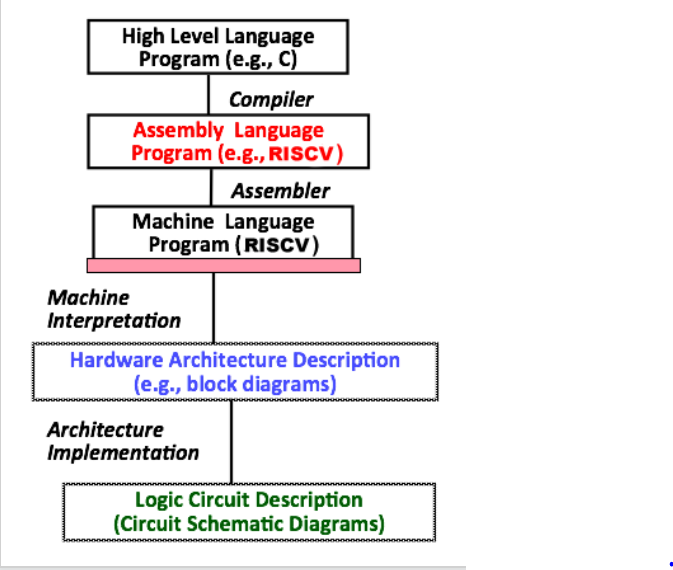
\includegraphics[]{abstraction}
\end{center}

\section{Intro to Assembly}
Assembly (or Assembly Languages or ASM) is a low-level programming language that maps a program's instructions to a particular architecture's operations. A low-level programming language is defined as a language with minimal abstraction from the architecture's (or computer's) instruction set. In summary, the Assembly language translates our C code to a set of instructions that the computer actually understands.

There are a few questions you may have about Assembly Languages at this point. One of those questions is how does the computer handle more complex operations from C, such as loops or other complex processes. The theory behind Assembly Languages in modern computing is that \textbf{instructions should be as simple and small as possible to optimize speed.} This theory is known as Reduced Instruction Set Computing, also known as \textbf{RISC}. This means that complex operations in C get translated to a set of very simple, minimal individual instructions.

Another potential question about Assembly languages that I personally had during this lecture was "aren't most computers different in some way from other computers? How do assembly languages work across different computers?" Well the answer to this question is shockingly simple. Assembly languages differ across computers. Since ASMs are designed specifically for the particular computer's architecture, they are not portable across machines like C or other higher level programming languages are. A generalization is that higher-level programming languages are the same across all computers, while low-level programming languages are specific for one computer.

This class will focus on the RISC-V assembly language. Many assembly languages have many similarities to each other, but \textbf{RISC-V} is what this class will use as it is one of the simpler ASMs out there with the smallest instruction sets.

\section{Registers}
Assembly languages do not have variables like C and other high-level programming languages do. Instead, Assembly languages store values in \textbf{Registers}, which are fixed, small spaces in memory (32 bit in this class). Our systems also have a limited number of these registers, but we use them since they are very fast and low power to access and change.

\subsection{Registers vs Memory}
Since there are a limited number of registers (only 32 available in our systems), it is very possible and likely that we will exceed our number of available registers. The computer handles this by \textit{spilling}, or moving some registers into the computer's memory. Registers are prioritized by keeping the most frequently used ones in the registers, and less used registers in the memory since accessing registers is much faster than accessing memory.

It is actually amazing how much faster accessing registers is than accessing memory (approximately 100 to 500 times faster).

We denote registers either by their number (ranges from x0 to x31), or by their name (s0 to s11 or t0 to t6). The s registers hold programmer's variables, which t registers hold temporary variables for the machine to handle.

\textbf{IMPORTANT CONCEPT:} registers in C have no type. The contents of a register are treated depending on the operation used.

\section{RISC-V Code}
All RISC-V instructions have the \textbf{exact} same, rigid syntax: 

\begin{center}
op dst, src1, src2
\end{center}

op=operation name, dst=destination register, src1=first source register, src2=second source register.

This regularity keeps things simple and fast for the hardware to handle.

RISC-V only has one operation per instruction, and one instruction per line. Here is a sample of a full assembly for the fibonnaci sequence:
\begin{center}
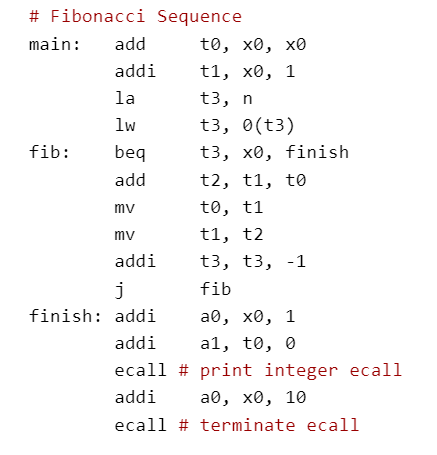
\includegraphics[]{assembly}
\end{center}

We have a reference sheet for all specific RISC-V assembly instructions. This class will focus on the various \textbf{types} of instructions and how they behave.

\section{Arithmetic}
The simplest instructions for us as programmers to understand. These commands, such as \textit{add} and \textit{sub} are just simple instructions for addition and subtraction. This translates almost directly from C code. These expressions only work when using them one two variables, wether they are variables from the code or temporary variables.

\section{Immediates}
These instructions are similar to the basic arithmetic instructions. With immediates, we are doing arithmetic on variables with specific integers, such as incrementing a variable by one. The basic syntax is the following:

\begin{center}
opi dst, src, imm
\end{center}

Note: the immediate must always be the second source, and the operations for immediates always end in an i.

Example operation:

\begin{center}
addi s1, s2, 5
\end{center}

\section{Data Transfer}
At this point, we understand that C variables map directly on to registers. Now we might ask, what about for large data structures, such as arrays or other structs? Well, these large data structures would be placed in the memory. However, RISC-V instructions only work on registers. So the question now is how does RISC-V perform operations on things stored in memory?

The answer to this question is that RISC-V has specific operations to move values to and from memory. In general, store operations moves values from the register to the memory, while load operations move values from the memory to the register.

Here is the basic syntax for data transfer operations:

\begin{center}
    memop reg, off(bAddr)
\end{center}

memop=memory operation, reg=register to perform operation on, bAddr=base address that points to somewhere in the memory, off=offset in bytes from the base address (this value can be an immediate). This means we access the memory at address bAddr+off

\textbf{IMPORTANT NOTE:} memory in assembly languages are byte addressed, similar to C. However, pointer arithmetic is not done for us. This means we must take the data size in to account when moving across an array.

RISC-V is also Little Endian, or the address of a word points to the least significant bit and increasing address points to increasingly significant bit.

\section{Control Flow}
Control flow is defined as statements that control if a block of code will be executed or how many times a block of code will be executed. We know these statements as comparative statements or loops in C.

RISC-V doesn't have code blocks, so these statements are done with labels. You will see these in RISC-V instructions with some text followed by a colon (ex. main:). Text that has control flow in RISC-V will have its own label for a certain set of instructions.

\section{End Note}
Familiarize yourself with the Green Reference sheet for RISC-V instructions. If there were any points that I may not have had time to cover in this note, check the lecture slides followed by asking for help on Piazza or Office Hours. Practice will make perfect for Assembly Languages, so give good effort on classwork related to Assembly.
\end{document}

